\documentclass{homework}

\title{CH5170 Assignment-1}
\author{S. VISHAL (CH18B020)}

\begin{document}

\maketitle
\section{Problem Details}
\begin{figure}[ht]
\centering
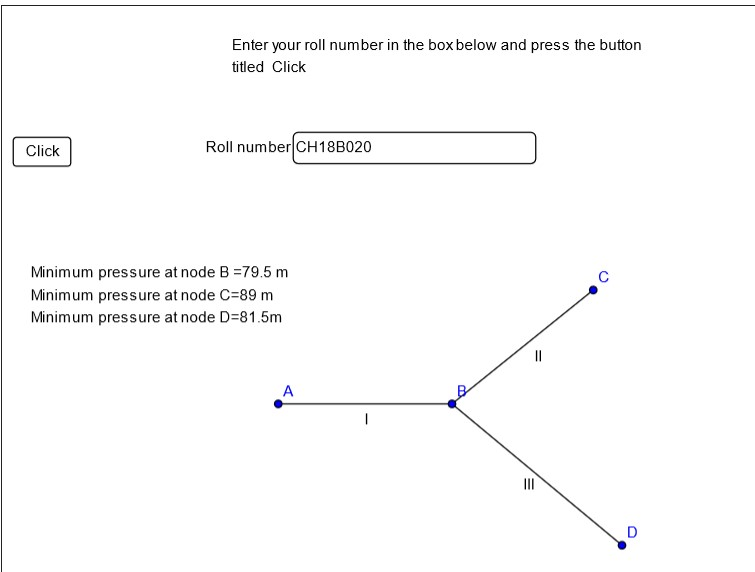
\includegraphics[width=0.75\textwidth]{question.jpg}
\caption{Pressure Values obtained from Geogebra}
\end{figure}
Other data as obtained from the Problem Sheet are:
\begin{enumerate}
\item $H_A$ = 100 m
\item Lengths of the links $L_{1}$ = 300 m, $L_{2}$ = 500 m, $L_{1}$ = 400 m. \item Flow rates in the links are $Q_1$ = 9 m$\m^3$/min, $Q_2$ = 3 m$\m^3$/min and $Q_3$ = 2 m$\m^3$/min respectively.
\end{enumerate}
Finally, cost of a pipe can be estimated using:
\begin{equation}\label{pipe_cost}
c = 1.2654LD^{1.327}
\end{equation}
where L is the length of the pipe (in m), and D is the diameter of the pipe (in mm)
\exercise*[1: Head Losses]
We make use of the following expression for head loss:
\begin{equation}\label{head_loss}
\Delta H = 4.457*10^8*\frac{LQ^{1.85}}{D^{4.87}}
\end{equation}
We can first write the equation at node B as:
\begin{equation}\label{node_B_Pressure}
H_A - H_B = 4.457*10^8*\frac{L_1Q_1^{1.85}}{D_1^{4.87}}
\Rightarrow{H_B = H_A - 4.457*10^8*\frac{L_1Q_1^{1.85}}{D_1^{4.87}}}
\end{equation}
For node C,
\begin{equation}\label{node_C_Pressure}
H_B - H_C = 4.457*10^8*\frac{L_2Q_2^{1.85}}{D_2^{4.87}}
\end{equation}
Substituting from \ref{node_B_Pressure} we get $H_C$ as:
\begin{equation}\label{node_C_Psub}
H_C = H_A - 4.457*10^8*\frac{L_1Q_1^{1.85}}{D_1^{4.87}}-4.457*10^8*\frac{L_2Q_2^{1.85}}{D_2^{4.87}}
\end{equation}
Proceeding similarly for node D:
\begin{equation}\label{node_D_Pressure}
H_B - H_D = 4.457*10^8*\frac{L_3Q_3^{1.85}}{D_3^{4.87}}
\end{equation}
\begin{equation}\label{node_D_Psub}
\Rightarrow H_D = H_A - 4.457*10^8*\frac{L_1Q_1^{1.85}}{D_1^{4.87}}-4.457*10^8*\frac{L_3Q_3^{1.85}}{D_3^{4.87}}
\end{equation}
Thus we have 3 equations (\ref{node_B_Pressure}, \ref{node_C_Psub} and \ref{node_D_Psub}) which relate the Head losses to some known parameters and the pipe diameters($D_1$, $D_2$ and $D_3$).
\exercise*[2: Total Cost]
We can simply use cost equation (eqn \ref{head_loss}) for all the three pipes:

Cost of link 1 (diameter $D_1$ and length $L_1$) is $c_1L_1 = 1.2654L_1D_1^{1.327}$

Cost of link 2 (diameter $D_2$ and length $L_2$) is $c_2L_2 = 1.2654L_2D_2^{1.327}$

Cost of link 3 (diameter $D_3$ and length $L_3$) is $c_3L_3 = 1.2654L_3D_3^{1.327}$

Adding them up we get,
\begin{equation}\label{Total_cost}
Cost = 1.2654L_1D_1^{1.327} + 1.2654L_2D_2^{1.327} + 1.2654L_3D_3^{1.327}
\end{equation}

\exercise[3: Cost in terms of Pressures]
Rearranging the Head Loss equation, and obtaining the diameter, we have from eqn \ref{head_loss}
\[D = (4.457*10^8*\frac{LQ^{1.85}}{\Delta{H}})^{\frac{1}{4.87}}\]
Proceeding same way for all 3 pipes we obtain:
\begin{equation}\label{D1}
D_1 = (4.457*10^8*\frac{L_1Q_1^{1.85}}{H_A-H_B})^{\frac{1}{4.87}}
\end{equation}
\begin{equation}\label{D2}
D_2 = (4.457*10^8*\frac{L_2Q_2^{1.85}}{H_B-H_C})^{\frac{1}{4.87}}
\end{equation}
\begin{equation}\label{D3}
D_3 = (4.457*10^8*\frac{L_3Q_3^{1.85}}{H_B-H_D})^{\frac{1}{4.87}}
\end{equation}
Substituting diameter values from equations \ref{D1},\ref{D2},\ref{D3} into the cost equation obtained previously (eqn \ref{Total_cost}), we obtain:

\begin{equation}\label{Cost_Head}
\begin{split}
Total cost = 1.2654*L_1*(4.457*10^{8}*\frac{L_1Q_1^{1.85}}{H_A - H_B})^{\frac{1.327}{4.87}} 
    & + 1.2654*L_2*(4.457 * 10^{8}*\frac{L_2Q_2^{1.85}}{H_B - H_C})^{\frac{1.327}{4.87}}
    & + 1.2654*L_3*(4.457 * 10^{8}*\frac{L_3Q_3^{1.85}}{H_B-H_D})^{\frac{1.327}{4.87}}
\end{split}
\end{equation}

\exercise*[4: Optimization Formulation]
Our objective is to minimize the cost function which we derived above.
The objective function:
\begin{equation}\label{Objective}
\begin{split}
Total cost = 1.2654*L_1*(4.457*10^{8}*\frac{L_1Q_1^{1.85}}{H_A - H_B})^{\frac{1.327}{4.87}} 
    & + 1.2654*L_2*(4.457 * 10^{8}*\frac{L_2Q_2^{1.85}}{H_B - H_C})^{\frac{1.327}{4.87}}
    & + 1.2654*L_3*(4.457 * 10^{8}*\frac{L_3Q_3^{1.85}}{H_B-H_D})^{\frac{1.327}{4.87}}
\end{split}
\end{equation}
such that (Inequality constraints)
\begin{equation}\label{Ineqc}
\begin{split}
H_B \geq 79.5m\\
H_C \geq 89m   \\
H_D \geq 81.5m
\end{split}
\end{equation}
And the diameters so obtained should be positive. (bound constraint; which upon substituting in the diameter in terms of head-loss equation \ref{node_B_Pressure}, \ref{node_C_Pressure} and \ref{node_D_Pressure} implies $H_A > H_B, H_B > H_C$ and $H_B > H_D$)

\exercise*[5: Optimum Pressures]
From the inequality and equality constraints we can infer 2 things:$\\\\$
1. \textbf{Inequality constraint-1 is redundant:} $\\$
For water to flow to tanks C and D from B, we know that $H_B > H_C$ and $H_B > H_D.\\$
But $H_C > 89 and H_D > 81.5$ which are higher than the limit 79.5 m imposed on $H_A$ as we can see from eqn \ref{Ineqc}. Therefore, Inequality constraint-1 is redundant. Imposing $H_C > 89m$ itself ensures $H_B > 89m\\$
2. \textbf{Optimal values of $H_C$ and $H_D$:} $\\$
Consider the equation \ref{node_C_Pressure}
\[H_B-H_C = 4.457*10^8*\frac{L_2Q_2^{1.85}}{D_2^{4.87}}\]
Let $H_C$ be some 100 m. If I keep decreasing $D_2$, the pressure head also keeps falling. Lower the diameter, lower the cost. So we keep lowering the diameter until we hit the minimum value for $H_C$. At this point, we can't reduce pipe size and hence the pipe cost for link II can't be reduced further.$\\$
\textbf{Therefore, $H_C$ = 89m is the optimal Pressure at node C.}$\\$
\textbf{By a similar argument, $H_D$ = 81.5m is the optimal Pressure at node D.} $\\$
As a result of the above inferences, we can remove all the 3 inequality constraints (automatically satisfied). We can then substitute values of $H_C$ and $H_D$ in equation \ref{Cost_Head} as 89m and 81.5m. \\
Now the objective is 
\begin{equation}\label{Cost_Head}
\begin{split}
Total cost = 1.2654*L_1*(4.457*10^{8}*\frac{L_1Q_1^{1.85}}{H_A - H_B})^{\frac{1.327}{4.87}} 
    & + 1.2654*L_2*(4.457 * 10^{8}*\frac{L_2Q_2^{1.85}}{H_B - H_C})^{\frac{1.327}{4.87}}
    & + 1.2654*L_3*(4.457 * 10^{8}*\frac{L_3Q_3^{1.85}}{H_B-H_D})^{\frac{1.327}{4.87}}
\end{split}
\end{equation}
Where $H_B$ is the only unknown and there are no constraints.

\exercise*[6: Unconstrained univariate optimisation]
The above optimisation problem was solved in MATLAB and the solution was found to be $H_B = 95.204m$ \\ And of course, as mentioned earlier, $H_C = 89m$ and $H_D = 81.5m$. \\
The corresponding pipe diameters obtained by substituting Pressure Heads in the equations from part one. \\
Diameter values:
\[D_1 = 321.5947 mm\]
\[D_2 = 223.1900 mm\]
\[D_3 = 155.3124 mm\]
Cost = Rs. $2.1096 * 10^6$\\
\textbf{MATLAB CODE:}
    \begin{verbatim}
clear;
% minimise costs
sol = fmincon(@cost,90,-1,80);
cost_sol = cost(sol);
L1 = 300; L2 = 500; L3 = 400;
Ho = 100; beta = 89; gamma = 81.5;
Q1  = 9; Q2 = 3; Q3 = 2;
D1 = (4.457*10^8)^(1/4.87)*(L1*Q1^1.85/(Ho-sol))^(1/4.87);
D2 = (4.457*10^8)^(1/4.87)*(L2*Q2^1.85/(sol-beta))^(1/4.87);
D3 = (4.457*10^8)^(1/4.87)*(L3*Q3^1.85/(sol-gamma))^(1/4.87);
function f = cost(HA)
    L1 = 300; L2 = 500; L3 = 450;
    Ho = 100; beta = 89; gamma = 81.5;
    Q1  = 9; Q2 = 3; Q3 = 2;
    f = 1.2654*L1*(4.457*10^8)^(1.327/4.87)*((L1*Q1^1.85/(Ho-HA)))^(1.327/4.87);
    f = f + 1.2654*L2*(4.457*10^8)^(1.327/4.87)*((L2*Q2^1.85/(HA-beta)))^(1.327/4.87);
    f = f + 1.2654*L3*(4.457*10^8)^(1.327/4.87)*((L3*Q3^1.85/(HA-gamma)))^(1.327/4.87);
end
\end{verbatim}

\exercise*[7: Optimisation for the case of Discrete Diameters]
Pipes of only a certain set of diameters are available in the market.
Since we can use two pipes per link, I am going to use two closest diameter
pipes in series as mentioned in the \emph{'problem set 1.pdf'}. This helps us get as close to a single pipe cost as possible.(because larger pipe is costlier than the optimal, and smaller pipe is cheaper than optimal[but can't maintain constraint]) Also, we need to ensure that the pressure constraints are satisfied. \\\\
Let the first link have two pipes of lengths $l_{11}$ and $l_{12}$, and the corresponding diameters be $d_{11}$ and $d_{12}$. Similarly, we define $l_{21}$, $l_{22}$, $l_{31}$, $l_{32}$, $d_{21}$, $d_{22}$, $d_{31}$, $d_{32}$. \\\\
For link 1 the diameters are:\( d_{11} = 300 mm\) \(d_{12} = 350 mm\). \\
For link 2 the diameters are:\( d_{21} = 200 mm\) \(d_{22} = 250 mm\). \\
For link 3 the diameters are:\( d_{31} = 150 mm\) \(d_{32} = 200 mm\). \\\\
Since, we are now using two pipes per link the total cost equation (eq. \ref{Total_cost}) is suitably modified as:
\begin{equation}\label{NewCost}
\begin{split}
Cost = 1.2654l_{11}d_{11}^{1.327} + 1.2654l_{12}d_{12}^{1.327} \\
+ 1.2654l_{21}d_{21}^{1.327} + 1.2654l_{22}d_{22}^{1.327} \\
+ 1.2654l_{31}d_{31}^{1.327} + 1.2654l_{32}d_{32}^{1.327} \\
\end{split}
\end{equation}
Further we have the following equality constraints:
\begin{equation}\label{NewEC}
\begin{split}
 L_1 = l_{11} + l_{12} \Rightarrow l_{12} = L_1 - l_{11} \\
 L_2 = l_{21} + l_{22} \Rightarrow l_{22} = L_2 - l_{21} \\
 L_3 = l_{31} + l_{32} \Rightarrow l_{32} = L_3 - l_{31}  \\
\end{split}
\end{equation}
So we can simplify the cost (eq. \ref{NewCost}) to
\begin{equation}\label{FinalCost}
\begin{split}
Cost = 1.2654l_{11}d_{11}^{1.327} + 1.2654(L_1 - l_{11})d_{12}^{1.327} \\
+ 1.2654l_{21}d_{21}^{1.327} + 1.2654(L_2 - l_{21})d_{22}^{1.327} \\
+ 1.2654l_{31}d_{31}^{1.327} + 1.2654(L_3 - l_{31})d_{32}^{1.327} \\
\end{split}
\end{equation}
We can write equations relating pressure and diameter similar to those in \ref{node_B_Pressure}, \ref{node_C_Psub}, \ref{node_D_Psub}. They come out to be:
\begin{equation}\label{HB}
H_B = H_A - 4.457*10^8*(\frac{l_{11}Q_1^{1.85}}{d_{11}^{4.87}} + \frac{l_{12}Q_1^{1.85}}{d_{12}^{4.87}})
\end{equation}\label{HC}
\begin{equation}
H_C = H_A - 4.457*10^8*(\frac{l_{11}Q_1^{1.85}}{d_{11}^{4.87}} + \frac{l_{12}Q_1^{1.85}}{d_{12}^{4.87}} + \frac{l_{21}Q_2^{1.85}}{d_{21}^{4.87}} + \frac{l_{22}Q_2^{1.85}}{d_{22}^{4.87}})
\end{equation}
\begin{equation}\label{HD}
H_D = H_A - 4.457*10^8*(\frac{l_{11}Q_1^{1.85}}{d_{11}^{4.87}} + \frac{l_{12}Q_1^{1.85}}{d_{12}^{4.87}} + \frac{l_{31}Q_2^{1.85}}{d_{31}^{4.87}} + \frac{l_{32}Q_2^{1.85}}{d_{32}^{4.87}})
\end{equation}
Then substituting the equality constraints in \ref{NewEC} and after some simplification, we can express the inequalities in \ref{Ineqc} in terms of $l_{11}$, $l_{21}$, and $l_{31}$. Notice that the equations are linear in the lengths, so we can express them in $Ax \leq B$ form.

\begin{equation}\label{finalineq1}
\begin{split}
(4.457*10^8)*
\begin{bmatrix}
Q_1^{1.85}/d_{11}^{4.87}-Q_1^{1.85}/d_{12}^{4.87} & 0 & 0 \\
Q_1^{1.85}/d_{11}^{4.87}-Q_1^{1.85}/d_{12}^{4.87} & Q_{2}^{1.85}/d_{21}^{4.87}-Q_2^{1.85}/d_{22}^{4.87} & 0 \\
Q_1^{1.85}/d_{11}^{4.87}-Q_1^{1.85}/d_{12}^{4.87} & 0 & Q_{3}^{1.85}/d_{31}^{4.87}-Q_3^{1.85}/d_{32}^{4.87} \\
\end{bmatrix}
*
\begin{bmatrix}
l_{11} \\ l_{21} \\ l_{31}
\end{bmatrix}
\\ =
\begin{bmatrix}
(H_A-79.5) - L_1*Q_1^{1.85}/d_{12}^{4.87}*(4.457*10^8) \\
(H_A-89) - L_1*Q_1^{1.85}/d_{12}^{4.87}*(4.457*10^8) - L_2*Q_2^{1.85}/d_{22}^{4.87}*(4.457*10^8) \\
(H_A-81.5) - L_1*Q_1^{1.85}/d_{12}^{4.87}*(4.457*10^8) - L_3*Q_3^{1.85}/d_{32}^{4.87}*(4.457*10^8)
\end{bmatrix}
\end{split}
\end{equation}
We further impose that the lengths should be physically meaningful, that is
\begin{equation}\label{finalineq2}
 0 \leq l_{k1} \leq L_k  
\end{equation}
for $k \in \{1,2,3\}$ $\\\\$
In summary we have the cost function (eqn \ref{FinalCost}) and the inequality constraints in (eqns \ref{finalineq1} and \ref{finalineq2}). This system was optimised in MATLAB and the solutions came out to be: \\\\
$l_{11} = 0m$ $l_{12} = 300m$ \\ $l_{21} = 303.206m$  $l_{22} = 196.7940m$ \\ $l_{31} = 370.223m$  $l_{32} = 29.7771m$\\\\ and the head losses were $\\$
$H_B = 96.8238m$ \\
$H_C = 89m$ \\
$H_D = 81.5m$\\\\
Expected Cost = Rs. $2.1908*10^6$
\subsection*{Inferences}
\begin{enumerate}
    \item We notice that $H_C$ and $H_D$ are the same as in the previous part! This is because, the arguments made earlier regarding the head losses are still valid here, and hence the 2 pressures are at their respective limiting values.
    \item Also, as expected, the cost is more in this case. If it wasn't then we would've obtained that solution in the previous case. So through proof by contradiction we have the cost always to be more in this case(we have imposed the additional constraint of restricting diameters to certain values).
\end{enumerate}
\subsection*{MATLAB CODE:}
    \begin{verbatim}
clear;
L1 = 300; L2 = 500; L3 = 400;
Ho = 100; beta = 89; gamma = 81.5; alpha = 79.5;
Q1  = 9; Q2 = 3; Q3 = 2;
d11 = 300; d12=350;
d21 = 200;d22 = 250;
d31 = 150; d32 = 200;
% LHS of the linear inequality constraint
A = zeros(9,3);
A(1,:) = [Q1^1.85/d11^4.87-Q1^1.85/d12^4.87 0 0]*(4.457*10^8);
A(2,:) = [Q1^1.85/d11^4.87-Q1^1.85/d12^4.87 Q2^1.85/d21^4.87-Q2^1.85/d22^4.87 0]*(4.457*10^8);
A(3,:) = [Q1^1.85/d11^4.87-Q1^1.85/d12^4.87 0 Q3^1.85/d31^4.87-Q3^1.85/d32^4.87]*(4.457*10^8);
A(4:6,:) = eye(3);
A(7:9,:) = -1*eye(3);
% RHS
B = zeros(9,1);
B(1) = (Ho-alpha) - L1*Q1^1.85/d12^4.87*(4.457*10^8);
B(2) = (Ho-beta) - L1*Q1^1.85/d12^4.87*(4.457*10^8) - L2*Q2^1.85/d22^4.87*(4.457*10^8);
B(3) = (Ho-gamma) - L1*Q1^1.85/d12^4.87*(4.457*10^8) - L3*Q3^1.85/d32^4.87*(4.457*10^8);
B(4) = L1; B(5) = L2; B(6) = L3;

% minimise costs
sol = fmincon(@cost,[0;300;400],A,B);
cost_sol = cost(sol);
% verification of solution
HA = Ho - 4.457*10^8*Q1^1.85*(sol(1)/d11^4.87 + (L1-sol(1))/d12^4.87);
HB = HA - 4.457*10^8*(Q2^1.85*(sol(2)/d21^4.87 + (L2-sol(2))/d22^4.87));
HC = HA - 4.457*10^8*(Q3^1.85*(sol(3)/d31^4.87 + (L3-sol(3))/d32^4.87));
function f = cost(x)
    L1 = 300; L2 = 500; L3 = 450;
    d11 = 300; d12=350;
    d21 = 200;d22 = 250;
    d31 = 150; d32 = 200;
    f = 1.2654*(x(1)*d11^1.327+(L1-x(1))*d12^1.327);
    f = f+ 1.2654*(x(2)*d21^1.327+(L2-x(2))*d22^1.327);
    f = f+ 1.2654*(x(3)*d31^1.327+(L3-x(3))*d32^1.327);
end
\end{verbatim}
    
\end{document}
